\documentclass[letterpaper, oneside, 10pt]{report}
\usepackage[margin = 1.0in]{geometry}
\usepackage[nottoc,notlof,notlot]{tocbibind}
\usepackage[hidelinks]{hyperref}
\usepackage{graphicx}
\usepackage{amssymb}
\usepackage{epstopdf}
\usepackage{setspace}
\usepackage{wrapfig}
\usepackage{enumitem}
\usepackage{fancyhdr}
\usepackage{cite}
\usepackage{classicthesis}
\usepackage{caption}
\usepackage{subcaption}

\geometry{letterpaper}

\DeclareGraphicsRule{.tif}{png}{.png}{`convert #1 `dirname #1`/`basename #1 .tif`.png}

\setlength{\skip\footins}{0.8cm}
\setlength{\tabcolsep}{30pt}

% Title page parameters
\lhead{Andrew Lawson}
\title{\large COOPERATIVE 3-D MAP GENERATION USING MULTIPLE UAVS}
\author{
  \large
  Andrew Lawson \\
  University of Connecticut \\
  Computer Science and Engineering
}
\date{\large May 1, 2015}
\pagestyle{fancy}

\begin{document}

% Title page
\begin{titlepage}
  \maketitle
  \thispagestyle{empty}
\end{titlepage}
\clearpage

% Abstract
\begin{abstract}

\noindent This report aims to demonstrate the feasibility of building a global 3-D map from multiple UAV robots in a GPS-denied, indoor environment. Presented are the design of each robot and the reasoning behind choosing its hardware and software components, the process in which a single robot obtains a individual 3-D map independently of external communication, and lastly how the mapping concept is extended to multiple robotic agents to form a global 3-D map using a centralized server. In the latter section, this report focuses on two algorithms, \textsl{Online Mapping} and \textsl{Map Fusion}, developed to facilitate the cooperative approach. A limited selection of experiments and test results are also presented to demonstate application of these algorithms in a real-world setting.

\end{abstract}
\clearpage

\renewcommand{\abstractname}{Acknowledgements}
\begin{abstract}
 I'd like to thank Prof. Shalabh Gupta, Prof. Ashwin Dani, and Prof. Robert McCartney for their advice and support. I'd also like to thank Kris Balisciano, Chung Yang, and everyone in L.I.N.K.S. Lab for all their work on the project.
\end{abstract}
\clearpage

% Table of Contents, Figures, and Tables
\tableofcontents
\listoffigures
\listoftables
\clearpage

\doublespacing

\chapter{Introduction}

\section{Overview}

In the modern field of robotics, the ability for a robot to move about the environment, regardless of the medium, has proven to be fairly trivial. However, the ability for a robot to track its own position and make deterministic decisions about it's own location in a foreign environment remains a fundamental, but critical problem. In most typical robotic experiments, the use of external measurement systems (such as GPS or motion capture cameras) allows researchers to capture the exact position of a robot in its environment and focus on other areas of interest. In the past couple decades, successful algorithms called SLAM\footnote{Simultaneous-Localization-And-Mapping: algorithm that uses sensor data to independently determine a position relational to an environment and simultaneously create a virtual map} have allowed singular robots to determine their own position in a world frame and construct a 3-D map from collected positional data. However, despite these advances, the ability for multiple UAV\footnote{UAV: unmanned aerial vehicle} robots to cooperatively determine their environmental boundaries is an area that remains relatively under-developed. By taking this cooperative approach with multiple robots, teams of coordinated robots could efficiently explore unaccessible areas, complete team-based tasks (like lifting large objects), conduct dangerous search and rescue missions, etc. This report explores the feasibility of mapping an indoor environemnt using multiple UAV robots where external positioning systems are not available. It should be noted that the navigation component of a robot using a SLAM system was not the focus of this project - the experiments and algorithms within instead concentrate on the computational and communicative aspects of developing a global map in such an environment.

\section{Literature Review}

In recent research projects with quadcopters, a wide variety of methods have been used to localize a robot in their environment, including (but not limited to) the use of high-resolution laser scanners \cite{bachrach2011range,shen2011autonomous}, monocular cameras \cite{soundararaj2009autonomous}, and ``RGB-D"\footnote{RGB-D: red-blue-green-depth} cameras as a combination of the two \cite{huang2011visual}. A laser has been used to generate a point cloud and pull out contours that trace the environment\cite{bachrach2011range}, a monocular camera to exploit texture gradients and continuations that can translated into depth estimates \cite{soundararaj2009autonomous}, and Microsoft Kinects (RGB-D cameras) to associate laser depth with image data \cite{huang2011visual}. Lasers capable of such precision and frequency are economically infeasible, and additionally, a pure laser approach is slow, can result in large margins of error, and lacks precision. Using a combination of the two, by means of an RGB-D camera, is responsive,  inexpensive, and produces results of reasonable reliability.


With previous RGB-D camera approaches, there have been five primary components: feature extraction, rotation estimation, feature matching, inlier detection, and motion estimation \cite{huang2011visual}. This involves taking certain features (like color, edges, corners, etc.) out of an image frame, estimating the rotation pose of the robot, matching new features to existing ones, filtering out bad data, and then estimating the motion of the robot. Using a data filter called an Extended-Kalman-Filter, the visual odometry data will be combined with velocity estimates to form a state estimation of the robot \cite{huang2011visual}. By implementing this filter, this will allow real-time positional estimates of the vehicle.


In recent years, researchers have attempted cooperative mapping methods similar to what's discussed in this report. Walter et al. showed experiments using cooperative SLAM in underwater vehicles \cite{walter2004experimental}. Riazuelo et al. developed the $C^{2}TAM$ cloud framework for cooperative tracking and mapping using UAVs \cite{riazuelo2014c}, where mapping and optimization is computed in the cloud. A few researchers have even demonstrated de-centralized SLAM methods, but either do not provide total three-dimensional capability or use external positioning sensors. For instance, Leung et al. used a VICON camera system \cite{leung2012decentralized} to provide true location data to decentralized robotic agents. Cunningham et al. implemented truly autonomous decentralized SLAM, but only focused on 2-D, planar data analysis \cite{cunningham2012large}.

This project attempts to build on this precedent by demonstrating cooperative mapping with UAVs as opposed to ground or aquatic robots. In addition, the mapping process is computed completely onboard the robot (as opposed to the cloud) and a centralized server is only used with the introduction of the cooperative component. Lastly, the robots used in this report are capable of building and communicating a completely three dimensional map as opposed to 2.5D or completely two dimensional data.

\chapter{Robot Design}

\section{Design Decisions}

Several key design decisions arose when choosing a direction for robot design and selection of components. The most signifcant choice for the robot was choosing an architecture for the onboard computational unit - specifically an ARM or x86 computer. The second key design dilemma (as mentioned briefly in the literature review) involved the selection of a laser-scanning sensor or an RGB-D camera. As shown below, both these choices had great effect upon the path of experimentation and results obtained.

\subsection{ARM vs. x86}

The main advantage of choosing an x86 board (found in most desktop or laptop computers) is compatibility. Almost all software packages are available in prebuilt, binary form on package managers (such as Ubuntu's apt-get) and setting up the computing environment can be done with a few simple installation commands. This convenience, unfortunately, comes at a financial and dimensional price - most small form-factor x86 boards are extremely expensive and cheaper options are considerably larger in size. These tradeoffs make selection of such a board unfeasible for an aerial drone where space is extremely limited and minimization of cost is a primary concern. As a result, ARM boards (like those in smartphones) are much more attractive - they offer extremely small form-factors, yet remain very affordable. The issue that arises, of course, is that of compatibility - many programs or libraries are not (immediately) available on an ARM installation and require manual compilation of source code using an ARM-based compiler and possible changes to the source code itself first. For this project, an ARM board was selected for the reasons listed above.

\subsection{Laser vs. RGB-D Camera}

The two major choices of sensors for robotic vision are using a laser scanner or an RGB-D camera. Much like the x86 computers, lasers are a terrific choice when cost is not a concern - they have wide field of view (some providing between 270 and 360 degrees), can scan very quickly (40 scans per second), and have amidable range (around 30 meters). However, a single unit can cost upwards of five thousand dollars and using only depth data can result in a large accumulation of error. An RGB-D camera, like the Microsoft Kinect, are very cheap sensors in comparison (the Kinect only costing only \$99 per unit). Unlike the laser, these sensors provide both depth and camera image data and less error is produced as a result of the ability to track image features across frames. However, they are slower (maximum of 30 scans per second) and require sigificantly more bandwidth for data transmission. Due to cost and error concerns, an RGB-D camera was selected for the experiments in this report.

\section{Hardware}

\subsection{Components}

The hardware design of the robot was focused on using low-cost, off-the-shelf components (see Table \ref{tbl: components.}). The approximate cost of a built robot was \$894, significantly cheaper than pre-built alternatives such as the AscTec Pelican used at MIT \cite{bachrach2011range} and University of Washington \cite{bachrach2012estimation} with similar project requirements.

% Table of components used on robot
\begin{table}[h!]
  \centering
  \caption{Table of Components}
  \vspace{2mm}
  \begin{tabular}{l l l}
    \hline \hline
    \vspace{-2mm}
    Component & \multicolumn{1}{l}{Description} & \multicolumn{1}{l}{Cost} \\ [1ex]
    \hline
    & \\
    DJI F450 Frame & Chassis & \$200 \\
    DJI 1045 Propellers & Props & \$10 \\
    DJI 2212 Motors & Actuators & \$30 \\
    12V and 5V Regulators & Power Reg. & \$40 \\
    Zippy 2450 mAh LiPo & Battery & \$30 \\
    64GB ODROID XU3 & ARM SBU & \$240 \\
    Pixhawk PX4 & Controller & \$220 \\
    Microsoft Kinect & Visual Sensor & \$99 \\
    MaxSonar EZ0	& Sonar Sensor & \$25 \\
  \end{tabular}
  \label{tbl: components.}
\end{table}

The robot used a stock F450 frame from DJI, which was not modified in any way - all components were mounted on existing areas using screws or adhesive products.The onboard computational unit chosen was the ODROID XU3 by HardKernel, which has a 1.7Ghz quad-core Snapdragon CPU, 2GB DDR3 RAM, 64GB eMMC flash storage, USB 3.0, and draws 5A. Initially, the robot was equipped with a PandaBoard ES, possessing a 1.2Ghz dual core with 1GB DDR3 RAM, SD card storage, and drawing 3A. Due to low memory and high read/write latencies, the latter board struggled to bear the load of even a full Ubuntu installation and was replaced with the XU3. For the visual sensor, a stripped down Microsoft Kinect Model 1473 was mounted onto the quadcopter - removing the sensor housing reduced weight from a heavy 3 lb to a very nimble 100 g. A Pixhawk PX4 flight controller was also added to the system for actuation control - this allowed the focus of the project to remain on the mapping and flight components of the robot. To accomodate the 12V, 1A requirements of the Kinect and 5V, 5A of the ODROID, several power regulators were mounted and installed to the robot's power system. The entire system was powered by a single 2450 mAh LiPo battery.

\begin{figure}[h!]
 \caption{Photograph of finished quadcopter robot.}
 \centering
   \includegraphics[width=0.3\textwidth]{images/quadcopter}
\end{figure}

\section{Software}

\subsection{Overview}

There were a number of key components needed to develop a software architecture for the robot. ROS Hydro was selected as a software package to manage the communication, networking, and overall data representation used throughout the robot, RGBDSLAM\_V2 as an algorithm integrated with ROS to develop the 3-D map onboard the robot, and lastly, MAVROS was an additional ROS package that was used to communicate with the motor controller. The data flow between all the software components can be seen in the Appendix in Figure \ref{fig: data flow.}.

\subsection{RGBDSLAM\_V2}
\noindent In order to compute a 3D map, the quadcopter's onboard computer uses a type of algorithm called SLAM (simultaneous localization and mapping), which computes a map and keeps track of the robotic agent's pose relative to said map. Due to time constraints, it was decided that a proprietary SLAM algorithm was not an option and a previously developed software package was chosen instead. Due to its compatibility with ROS and extensive usage throughout the robotics community, RGBDSLAM\_V2 \cite{endres2012evaluation} was the software used to produce the map and pose transformations of the robot during flight.

% RGBDSLAM data flow
\begin{figure}[h!]
 \caption{Data flow of RGBDSLAM\_V2 \cite{endres2012evaluation}}
 \centering
   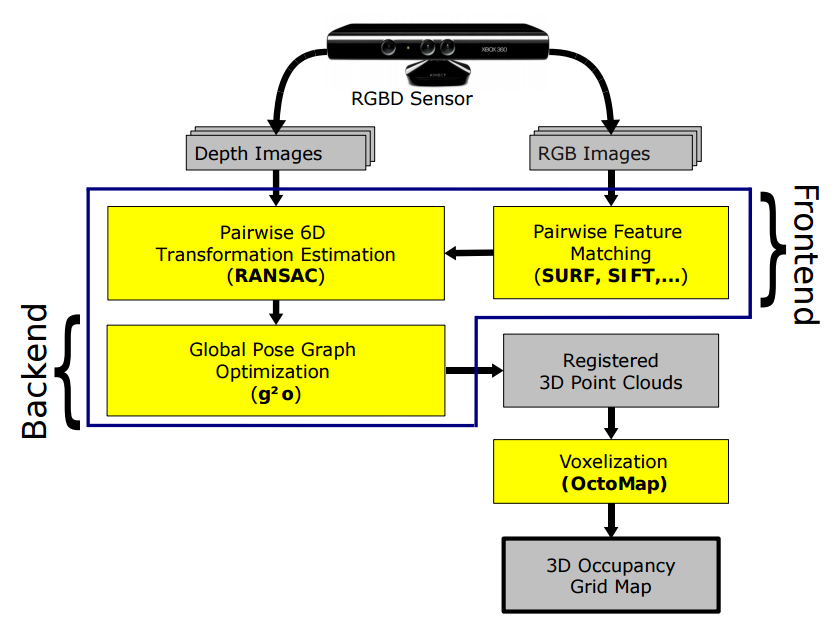
\includegraphics[width=0.6\textwidth]{images/rgbdslam}
 \label{fig: rgbdslam.}
\end{figure}

As opposed to sensors like a scanning laser, RGBDSLAM\_V2 provides a SLAM algorithm that can be interfaced with RGB-D sensors like the Microsoft Kinect used throughout this report. The backend of the algorithm consists of a pose graph, as seen in Figure \ref{fig: rgbdslam.}, where each node represents the 3-D pose of the sensor / robot and each edge corresponds to pairwise transformations between sensor poses in the pose graph. This graph is used in tandem with the depth and image data to produce the transformed point clouds in the output map.

\subsection{ROS Hydro}

Robot Operating System (ROS) is a meta operating system that is installed as package on a UNIX-based OS like Ubuntu or OS X. In a nutshell, ROS allows one to design their robot using a distributed model, where each ROS \textsl{node} is essentially a process or computational component of the robot. It also provides asynchronous and synchronous communication libraries, networking libraries, and supports multiple programming languages. Using said libraries, nodes can obtain information output from other nodes via a subscription or reply-request model as well as output  data themselves in the same fashion. Usage of ROS in the project allowed focus to remain on algorithm development and abstracts out the software glue that connects all the different algorithms running onboard.

% ROS architecture
\begin{figure}[h!]
 \caption{Photograph of finished quadcopter robot.}
 \centering
   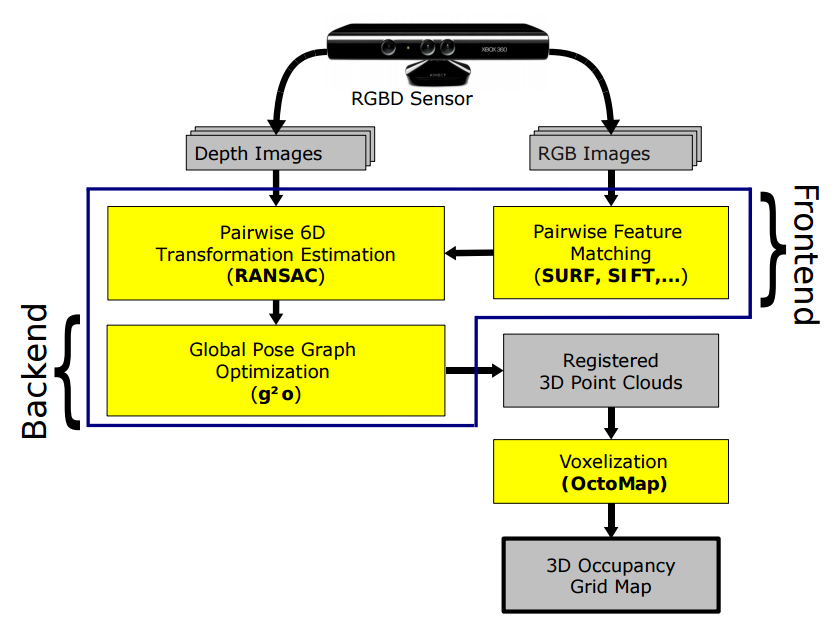
\includegraphics[width=0.3\textwidth]{images/rgbdslam}
\end{figure}

Within the system presented in the report, there were several nodes that partitioned the processes running in real time on the robot. RGBDSLAM produced the map and pose of the robot onboard, which were each broadcast to the server when running cooperative mapping. The Map Fusion node was also running on the server (discussed in a later section) which subscribed to said data and produced the global map for all the robots. MAVROS was used onboard the robot to take command requests from the onboard computer and send them to the Pixhawk controller.

\subsection{MAVROS}

In order for the onboard computer to communicate with the Pixhawk controller, it makes use of a ROS package called MAVROS. This runs as another ROS node in the ROS system which allows the computer to send commands to the Pixhawk from a high-level. This includes commands such as arming and disarming of the motors, take-off and landing commands, checking battery levels, and sending RC values to change the state of the motors (move).

%\begin{figure}[h!]
 %\caption{Prototype quadcopter.}
 %\centering
   %\includegraphics[width=0.6\textwidth]{copter}
%\end{figure}

MAVROS to communicates with the computer using a data protocol called MAVLINK - this allows a graphical user interface, such as that recommended by the Pixhawk manufacturer, to be used in tandem with MAVROS and that data that it publishes.

\chapter{Single Robot}

\section{Autonomy}
As the focus of this project is on the mapping component, fully-developed autonomous navigation is not present. However, some elements for inputless flight are implemented and provide a baseline for future work.

    \subsection{Pixhawk PID}
    The Pixhawk PX4 controller provides a built-in PID controller, which is used for drift stability and basic feedback control of the quadcopter. The proportional, integral, and derivative parameters were tuned through trial and error - adjusting each component until the quadcopter no longer oscillated and remained stable.

    \subsection{Altitude Control}

    The Pixhawk PX4 also provides an altitude holding system, given an input sensor.

\section{Mapping}

In a previous paper, Bachrach et al. implemented RGB-D mapping, and in a separate publication \cite{bachrach2011range}, laser mapping, by offloading realtime processing to a local server \cite{bachrach2012estimation}.  This robot design differs from its contemporaries by computing all steps of the mapping procedure onboard. As noted in Figure X, the quadcopter's onboard computer runs an RGBDSLAM ROS node in realtime during flight. This node generates the three-dimensional map, which can be be saved on disk as a file through a service call in ROS and retrieved after a test flight. The ROS node also allows requests for the current state of the map. As a result, a custom ROS node was written that allows for realtime visualization - this can be streamed to a nearby computer via Wi-Fi connection (see Figure X, Y). These two options allow for absolute flexibility in situations where remote access to the robot may or may not be possible.

\section{Results}
\noindent Testing of a single quadcopter robot was done in the concourse of the Information Technology Engineering building on the UConn Storrs campus. As seen in Figure 5, an image taken of the quadcopter in flight can be seen in the top left, the RGB stream from the Kinect sensor on the bottom left, and on the right-hand side, the 3-D map generated in realtime by the onboard computer.

% Map fusion algorithm flowchart
\begin{figure}[h]
 \caption{Live test of a single quadcopter.}
 \centering
   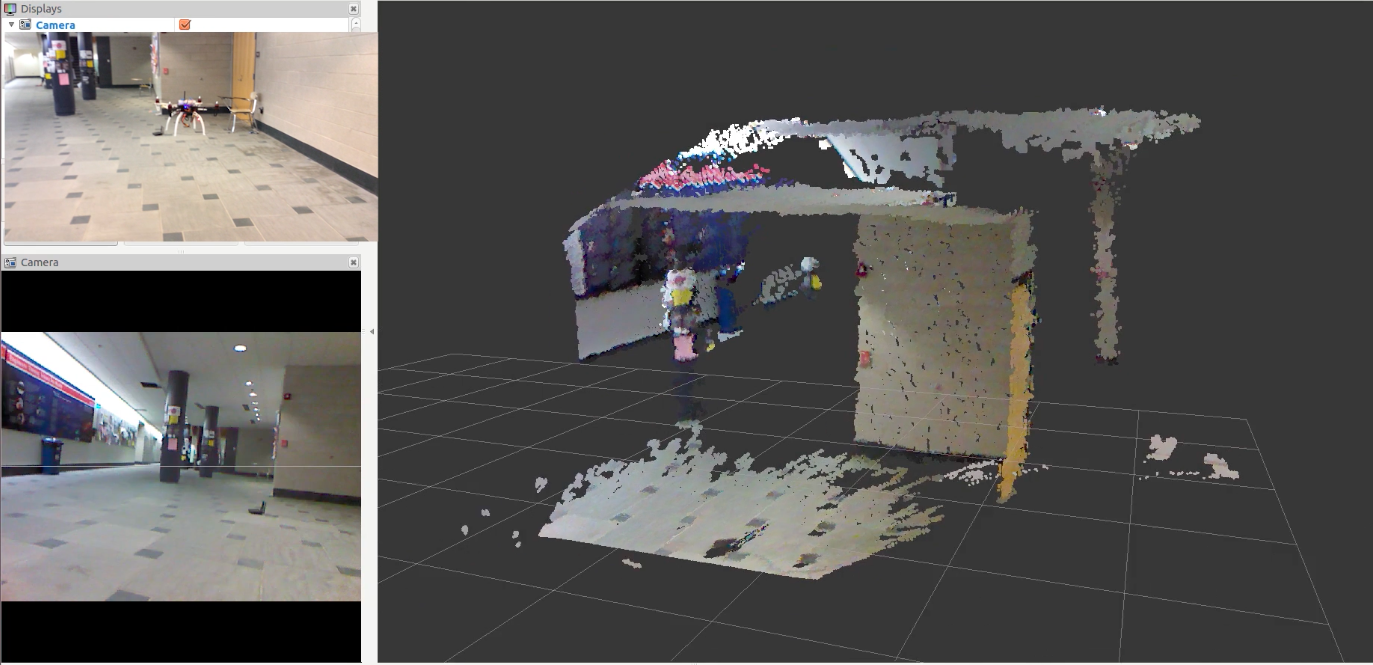
\includegraphics[width=0.8\textwidth]{images/single_test}
\end{figure}

\noindent Several repeated tests showed responsive mapping at about 7 frames per second. These maps were streamed in real time to a base station through a local wireless network.

\chapter{Multiple Robots}

\section{Overview}

When transitioning from one robotic agent creating its own map to generating a global 3-D map for multiple disjoint robot agents, it's essential to fuse each robot's maps together. This requires the introduction of a centralized, external server as the onboard computational units do not have the computing power to both generate the map for singular robot usage and to construct the cooperative map simultaneously in the case of multiple agents. The server's function is underlined by two key algorithms, first the \textsl{Online Mapping} algorithm which reconstructs each robot's map in real time as it sends timestamped point clouds over the network and second the \textsl{Map Fusion} algorithm, which fuses the the two aggregate disjoint maps together.

\section{Online Mapping}
As discussed in the overview, each quadcopter produces a point cloud segment which it sends over the network to be aggregated into a single map corresponding to that robotic agent. There are two primary methods to accomplish this, both with unique drawbacks. The first method is to deliver the entire aggregated point cloud map computed by RGBDSLAM at given intervals to the server - this becomes infeasible very quickly because as time grows, the size of the map will grow to hundreds of megabytes and current network speeds are unable to process such a load in a reasonable time frame. The other solution is to send each individual point cloud corresponding to a timestep over the network, resulting in a reconstruction of the map on the server. This is inefficient, because the map has already been built onboard and it is redundant to perform the same operation remotely. The experiments in this report used the latter method (despite its obvious weaknesses) given constraints and time restrictions of the project.

% Networked map building algorithm flowchart
\begin{figure}[h!]
 \caption{Data flow of online mapping algorithm.}
 \centering
   \includegraphics[width=0.8\textwidth]{images/online_streaming}
 \label{fig: online stream.}
\end{figure}

Coupled with the mapping component of the RGBDSLAM package, a custom ROS node was written (integrated with RGBDSLAM) that provided a stream of clouds added to the map to through a new ROS topic, each corresponding to new nodes added within the graph. As shown in Figure \ref{fig: online stream.}, these clouds and their respective transforms\footnote{The transform of the cloud is that between the RGB optical frame of the Kinect camera and the fixed frame of the robot's map.} are computed by RGBDSLAM, sent procedurally over the network, received by a server or other external computer, which then executes the online map builder algorithm for each cloud. The algorithm first matches the new cloud $\bf{P_n}$ with its transform $\bf{T_n}$ by performing a transformation lookup keyed by the timestamp $\bf{t_n}$ of the cloud (located in its header data). Once located, the transformation is applied to the cloud, changing its pose to be relative to the aggregate map $\bf{P_a}$. Once this transformation is applied, the new cloud can be simply appended to the current aggregate cloud in the simple operation $\bf{P_a} += \bf{P_n}$  - this new version of the cloud $\bf{P_a}$ is then saved into a database or filesystem.

\section{Map Fusion}
\noindent Once these aggregate maps corresponding to the robotic agents are reconstructed on the server, each map has its own point cloud and transformation in 3-D space. Unlike the \textsl{Online Mapping} algorithm, there is not a known transformation\footnote{In Online Mapping, the fixed frame is determined by the pose of the first cloud generated, so a transformation can be found from the camera frame of subsequent maps. In Map Fusion, no such initial transformation is known.} between the frames of the disjoint maps - this means the \textsl{Map Fusion} procedure must approximate the transformation between the two maps. Following a similar approach to Henry et. al.\cite{henry2012rgb}, the algorithm transforms two maps into the same global reference frame through several alignment approximations, stitches the maps together, and eliminates redundant data points by applying a voxel filtering algorithm. By incrementally applying the map fusion algorithm to the aggregate maps, the server outputs a timestamped representation of the global map. As shown in Figure 2, this algorithm is divided into two key sections.

% Map fusion algorithm flowchart
\begin{figure}[h!]
 \caption{Data flow of map fusion algorithm.}
 \centering
   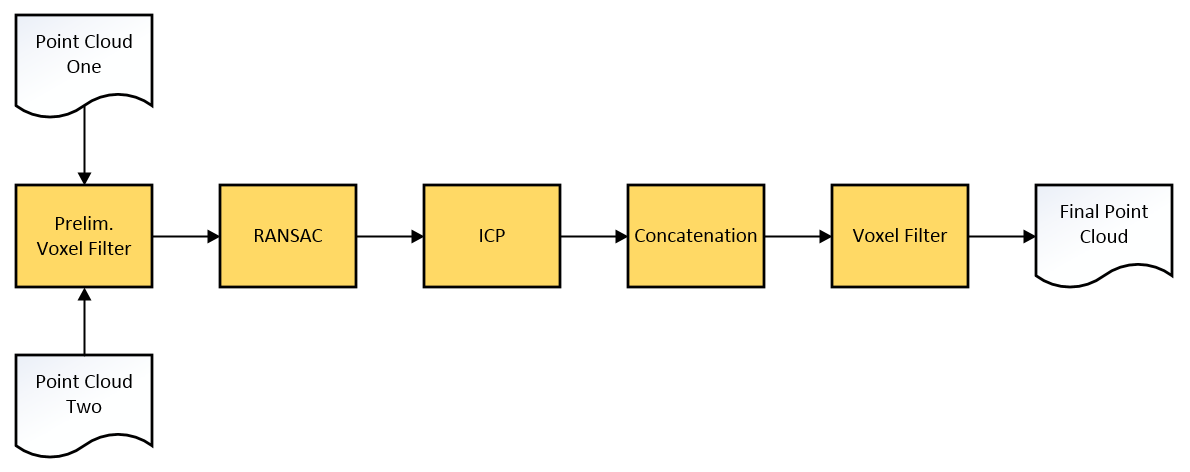
\includegraphics[width=0.9\textwidth]{images/mapfusion}
 \label{fig: map fusion.}
\end{figure}

    \subsection{Sample Consensus Initial Alignment}

    \noindent As mentioned in the overview, it's necessary to transform the source map into the reference frame of the target map, however, this process must be approximated through an iterative process. The point clouds are first put through an initial alignment phase that provides a rougher, larger-scale transformation estimation. This is done using the Sample Concensus Initial Alignment algorithm \cite{rusu2009fast}. from the Point Cloud Library. This process outputs a final transformation which is applied to the source cloud, as seen in Figure ~\ref{fig:Raw concatentation.}.

    \begin{figure}[h]
     \caption{Data flow of SCIA process.}
     \centering
       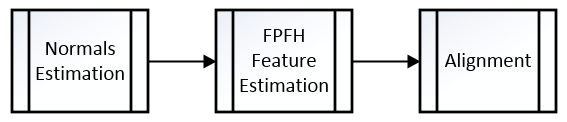
\includegraphics[width=0.45\textwidth]{images/initialalignment}
    \end{figure}

    \noindent Within the SCIA process itself, there are several subprocesses. First, the normals $N_{source}$ and $N_{target}$ are found by PCL's normal estimator. These normal clouds represent the estimated surface normals at each point in the cloud. They are then used in PCL's Fast Point Feature Histogram (FPFH) \cite{rusu2009fast,rusu2009fastlabel} estimator, to generate approximate feature clouds $F_{source}$ and $F_{target}$. These feature clouds store feature descriptors for each point in the cloud, in this case, FPFH features. Although, the theory behind image features is beyond the scope of this report, the FPFH feature approximates the mean curvature of a point's k-neighbors' geometry with a histogram of values - this type of feature allows computation of a feature cloud in asympototically linear time, giving a powerful but relatively quick feature estimator. Lastly, these feature clouds from this process are used to estimate an initial transformation $T$, which is applied to the initial source cloud to obtain an initial alignment. This gives the clouds a reasonably close placement relative to each other, and allowing optimal usage of second stage of alignment, ICP, to correct their positioning on a finer scale. The parameters used to tune the SCIA process can be seen in Table \ref{tbl: map fusion param.} within the Appendix.

    \subsection{Iterative Closest Point}

    \noindent After the clouds have passed through the initial alignment stage, they are locally optimized using the Iterative Closest Point algorithm. ICP takes a point cloud $P_{source}$ and finds the nearest k-neighbor points in $P_{target}$. By minimizing the sum of squares error, a rigid transformation $T$ between $P_{source}$ and $P_{target}$ is output. As shown in Figure ~\ref{fig:SCIA alignment.}, this transformation is applied to $P_{source}$ which eliminates narrower errors between the two clouds. The parameters used to tune the ICP process can be seen in Table \ref{tbl: map fusion param.} within the Appendix.

    \subsection{Filtering and Concatentation}

    Lastly, the target and transformed source cloud are concatenated using Point Cloud Library's concatentation features - programmatically, this is as simple as just adding the clouds together. Using another Voxel filter, the excess data points are trimmed away to generate the final stitched version of the map, as shown in Figure ~\ref{fig:ICP alignment.}. The parameters used to tune the filtering process can be seen in Table \ref{tbl: map fusion param.} within the Appendix. \\

% Map fusion visuals
\begin{figure}[h]
    \centering
    \begin{subfigure}[h]{0.31\textwidth}
        \centering
        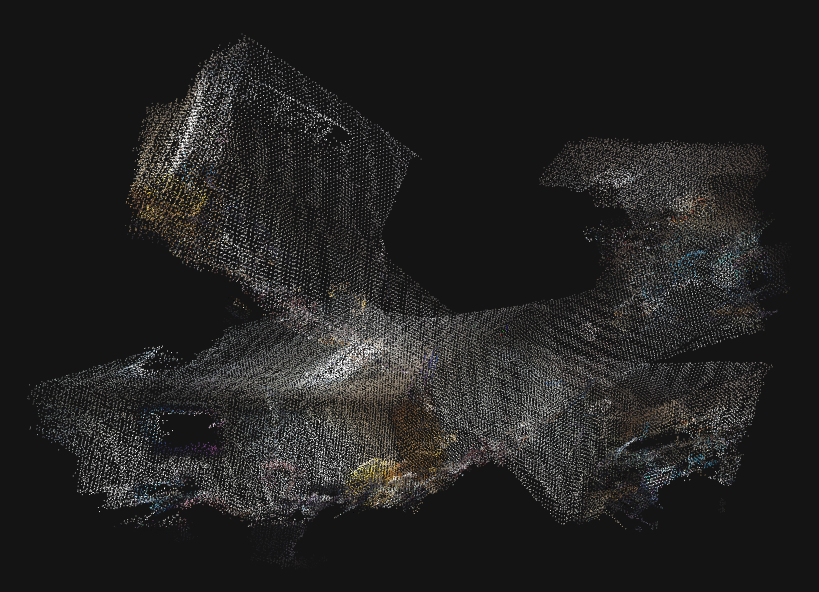
\includegraphics[width=\textwidth]{images/fusion_raw}
        \caption{Raw concatentation.}
        \label{fig:Raw concatentation.}
    \end{subfigure}
    \hfill
    \begin{subfigure}[h]{0.31\textwidth}
        \centering
        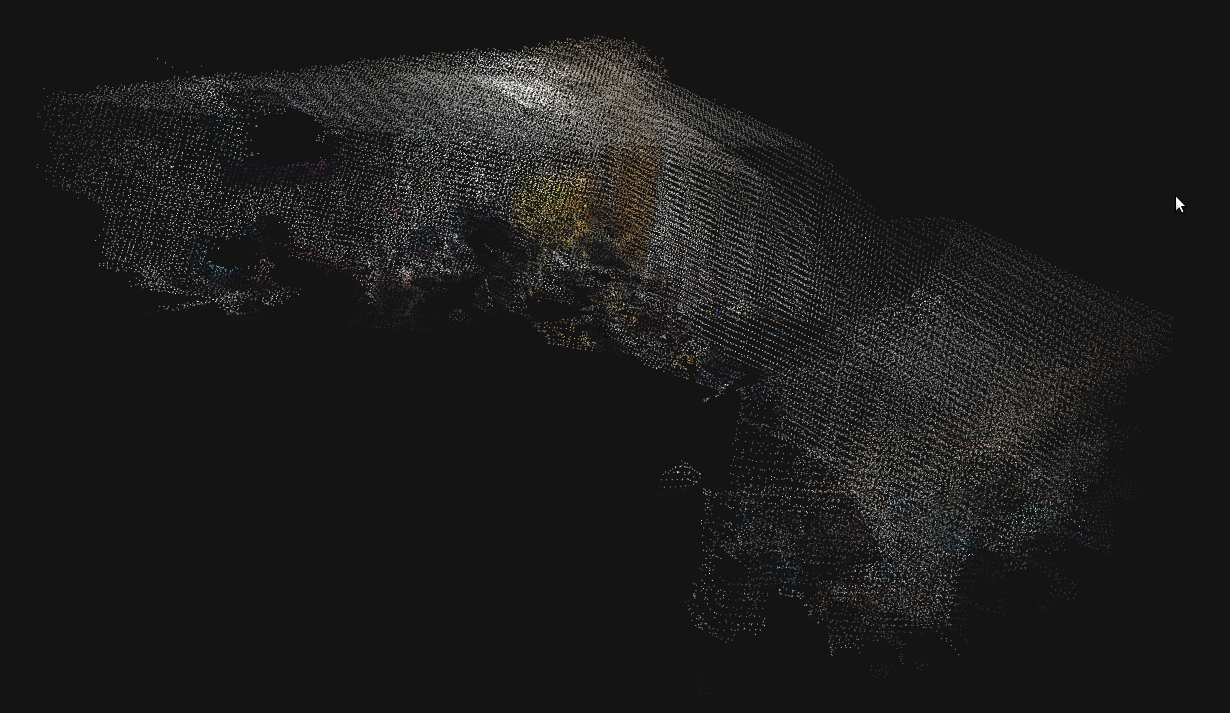
\includegraphics[width=\textwidth]{images/fusion_scia}
        \caption{SCIA alignment.}
        \label{fig:SCIA alignment.}
    \end{subfigure}
    \hfill
    \begin{subfigure}[h]{0.31\textwidth}
        \centering
        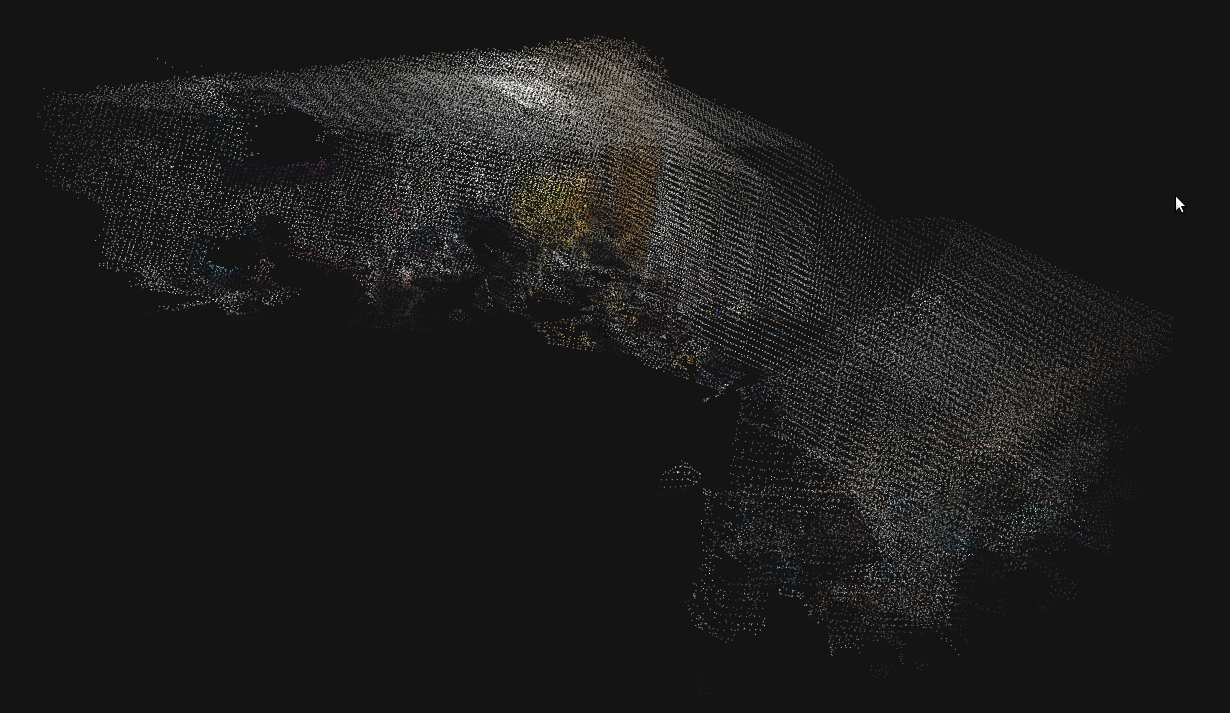
\includegraphics[width=\textwidth]{images/fusion_scia}
        \caption{ICP alignment.}
        \label{fig:ICP alignment.}
    \end{subfigure}
    \caption{Visual process of map fusion.}
    \label{fig:Visual process of map fusion.}
\end{figure}

\section{Results}

Due to financial and logistical difficulties, a test involving two quadcopters flying simultaneously in real time was unable to be conducted within the time frame for this project. As an alternative to demonstrate effectiveness of the approaches demonstrated in this report, two separate flights using the same quadcopter were conducted in the same environment and saved into ROS bags. These ROS bags were then simulated as live agents, with map data streaming at the same frequency and conditions as a real multi-robot flight test - this provided data to the map fusion server that exactly duplicates two quadcopters flying simultaneously and serves as an acceptable substitution for a real test.

A test was conducted in the L.I.N.K.S Lab, with a simple spinning motion to capture the depth and RGB data of the room. One half of the room was captured by the first robot and the second half of the room was captured by a second robot.

\chapter{Conclusions}

\subsection{Future Work}

As stated earlier, this project did not focus on navigation or control of multiple quadcopters and focused on the feasibility of mapping using multiple quadcopters. A natural progression forward would be to implement localization and possibly object avoidance algorithms in parallel with the mapping procedures. The RGBDSLAM algorithm in this report was used exclusively for its mapping and pose graph features, but was selected partly because of its capabilities of estimating trajectory and facilitating full autonomous navigation. Implementation of navigation in tandem with the concepts presented in this report would be a significant achievement.

In an optimal world, a centralized approach to cooperative mapping will not be necessary and the onboard computational units could cooperatively compute the global map, independent of external communication. It's clear that the application of such a concept is limited largely by technological capabilities. A possible solution to this problem could be to add a secondary computational unit aboard each robotic agent - this would allow for sufficient computational overhead to compute the global map in a decentralized manner, but would increase the power and weight requirements of the robot significantly, resulting in need of a larger capacity battery to compensate for increased thrust and power needs. This would, in turn, increase the weight of the quadcopter and reduce flight time.

\chapter{Appendix}

% Component data flow diagram
\begin{figure}[h!]
 \caption{Data flow of quadcopter components.}
 \centering
   \includegraphics[width=0.8\textwidth]{images/data_flow}
 \label{fig: data flow.}
\end{figure}

% Table of PID parameters
\begin{table}[h!]
  \centering
  \caption{PID Parameters}
  \vspace{2mm}
  \begin{tabular}{l l}
    \hline \hline
    \vspace{-2mm}
    Parameter & \multicolumn{1}{l}{Value} \\ [1ex]
    \hline
    & \\
    Proportional & 0.05 \\
    Integral & 0.1 \\
    Derivative & 50 \\
  \end{tabular}
\end{table}

% Table of Map Fusion parameters
\begin{table}[h!]
  \centering
  \caption{Map Fusion Parameters}
  \vspace{2mm}
  \begin{tabular}{l l}
    \hline \hline
    \vspace{-2mm}
    Parameter & \multicolumn{1}{l}{Value} \\ [1ex]
    \hline
    & \\
    Voxel Leaf Size & 0.05 \\
    ICP Max. Corresp. Dist. & 0.1 \\
    ICP Max. Iter. & 50 \\
    ICP Trans. Epsilon & 1e-8 \\
    ICP Euclid. Epsilon & 1 \\
    SCIA Min. Sample. Dist & 1 \\
    SCIA Max. Corresp. Dist & 1 \\
    SCIA Max. Iter. & 50 \\
  \end{tabular}
  \label{tbl: map fusion param.}
\end{table}

\clearpage

\bibliography{uscholar}
\bibliographystyle{ieeetr}

\end{document}
